\documentclass[tikz,border=8pt]{standalone}
\usepackage{amsmath,amssymb}
\usetikzlibrary{arrows.meta,automata,positioning,quotes}
\begin{document}
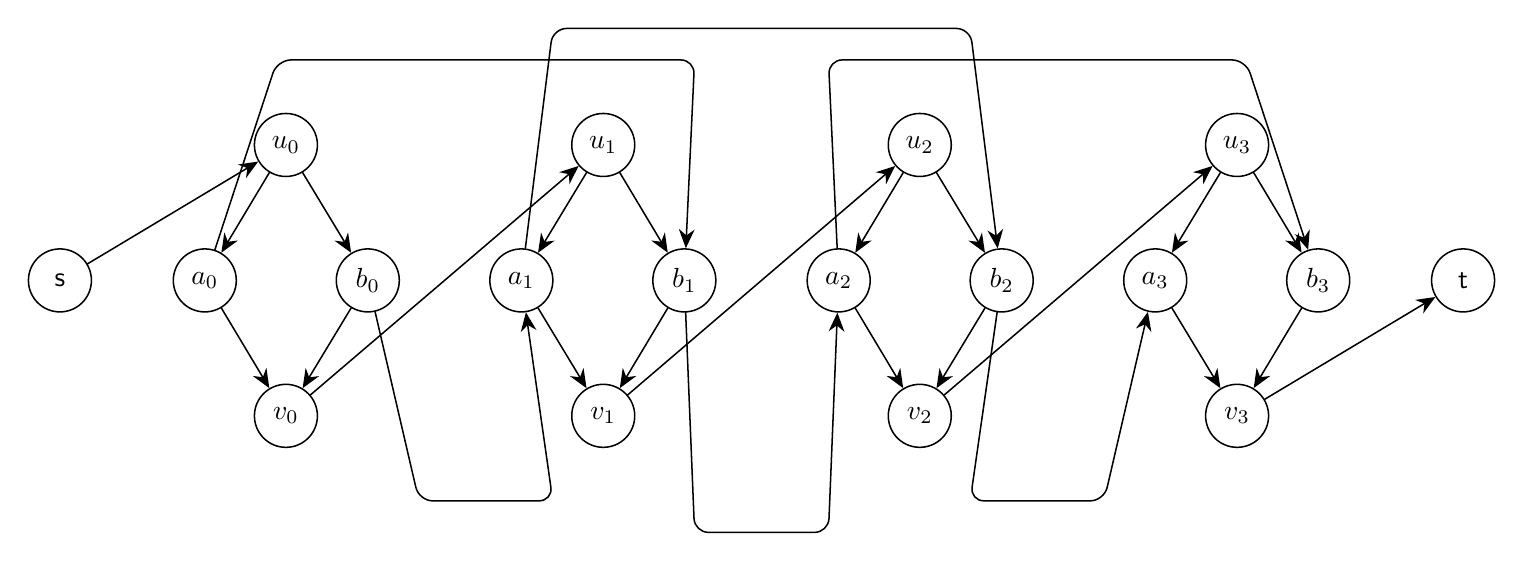
\begin{tikzpicture}[x=1cm,y=1cm]
\tikzset{
  graphnode/.style={circle,draw=black,line width=0.55pt,minimum size=8mm,inner sep=1pt,font=\sffamily},
  graphedge/.style={draw=black,line width=0.55pt,line cap=round,line join=round},
  directed/.style={graphedge,-{Stealth[length=2.4mm,width=2.0mm]}},
  undirected/.style={graphedge}
}
\node[graphnode] (n_s) at (-1.16,0.00) {s};
\node[graphnode] (n_t) at (16.66,0.00) {t};
\node[graphnode] (n_u_0) at (1.71,1.72) {$u_{0}$};
\node[graphnode] (n_v_0) at (1.71,-1.72) {$v_{0}$};
\node[graphnode] (n_a_0) at (0.68,0.00) {$a_{0}$};
\node[graphnode] (n_b_0) at (2.75,0.00) {$b_{0}$};
\node[graphnode] (n_u_1) at (5.74,1.72) {$u_{1}$};
\node[graphnode] (n_v_1) at (5.74,-1.72) {$v_{1}$};
\node[graphnode] (n_a_1) at (4.70,0.00) {$a_{1}$};
\node[graphnode] (n_b_1) at (6.77,0.00) {$b_{1}$};
\node[graphnode] (n_u_2) at (9.76,1.72) {$u_{2}$};
\node[graphnode] (n_v_2) at (9.76,-1.72) {$v_{2}$};
\node[graphnode] (n_a_2) at (8.73,0.00) {$a_{2}$};
\node[graphnode] (n_b_2) at (10.80,0.00) {$b_{2}$};
\node[graphnode] (n_u_3) at (13.79,1.72) {$u_{3}$};
\node[graphnode] (n_v_3) at (13.79,-1.72) {$v_{3}$};
\node[graphnode] (n_a_3) at (12.75,0.00) {$a_{3}$};
\node[graphnode] (n_b_3) at (14.82,0.00) {$b_{3}$};
\draw[directed] (n_u_0) -- (n_a_0);
\draw[directed] (n_u_0) -- (n_b_0);
\draw[directed] (n_a_0) -- (n_v_0);
\draw[directed] (n_b_0) -- (n_v_0);
\draw[directed] (n_u_1) -- (n_a_1);
\draw[directed] (n_u_1) -- (n_b_1);
\draw[directed] (n_a_1) -- (n_v_1);
\draw[directed] (n_b_1) -- (n_v_1);
\draw[directed] (n_u_2) -- (n_a_2);
\draw[directed] (n_u_2) -- (n_b_2);
\draw[directed] (n_a_2) -- (n_v_2);
\draw[directed] (n_b_2) -- (n_v_2);
\draw[directed] (n_u_3) -- (n_a_3);
\draw[directed] (n_u_3) -- (n_b_3);
\draw[directed] (n_a_3) -- (n_v_3);
\draw[directed] (n_b_3) -- (n_v_3);
\draw[directed] (n_s) -- (n_u_0);
\draw[directed] (n_v_0) -- (n_u_1);
\draw[directed] (n_v_1) -- (n_u_2);
\draw[directed] (n_v_2) -- (n_u_3);
\draw[directed] (n_v_3) -- (n_t);
\draw[directed,rounded corners=5pt] (n_a_0) -- (1.60,2.80) -- (6.90,2.80) -- (n_b_1);
\draw[directed,rounded corners=5pt] (n_b_0) -- (3.40,-2.80) -- (5.10,-2.80) -- (n_a_1);
\draw[directed,rounded corners=5pt] (n_a_1) -- (5.10,3.20) -- (10.40,3.20) -- (n_b_2);
\draw[directed,rounded corners=5pt] (n_b_1) -- (6.90,-3.20) -- (8.60,-3.20) -- (n_a_2);
\draw[directed,rounded corners=5pt] (n_a_2) -- (8.60,2.80) -- (13.90,2.80) -- (n_b_3);
\draw[directed,rounded corners=5pt] (n_b_2) -- (10.40,-2.80) -- (12.10,-2.80) -- (n_a_3);
\end{tikzpicture}
\end{document}
